
\section{Motivations}
\label{repl:sec:motivations}

\begin{figure*}
  \centering
  \subfloat[Document Wikipédia principalement édité en fin.]
  [Document Wikipédia de très grande taille principalement édité en fin.]
  {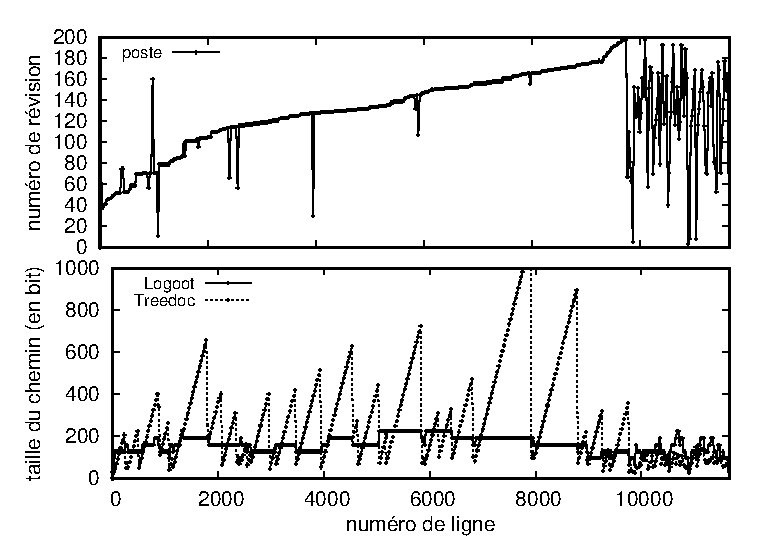
\includegraphics[width=0.8\textwidth]{img/lseq/motivationposte.eps}}
  \hspace{10pt}
  \subfloat[Document Wikipédia principalement édité au début.]
  [Document Wikipédia de petite taille principalement édité en début.]
  {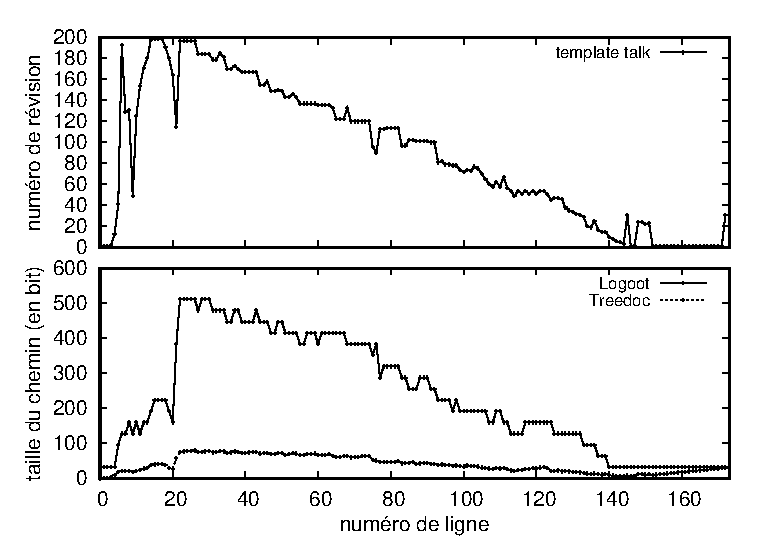
\includegraphics[width=0.8\textwidth]{img/lseq/motivationtemplatetalk.eps}}
  \caption{\label{repl:img:motivations}Motivations}
\end{figure*}

L'encyclopédie Wikipédia répertorie des millions d'articles écrits
collaborativement par sa communauté. Un utilisateur, enregistré ou non, peut
lire un article, et s'il le souhaite, en modifier le contenu. Lorsque ses
modifications sont achevées, il les soumet à Wikipédia. Deux issues possibles :
\begin{inparaenum}[(i)]
\item La contribution est acceptée et sera visible de tous ou
\item la contribution est rejetée car un autre utilisateur a effectué une
  modification en concurrence et l'a soumise en premier. Il faut alors réviser
  la version rejetée afin de l'adapter à la version la plus à jour avant de
  resoumettre si nécessaire.
\end{inparaenum}
Wikipédia garde l'historique des modifications apportées à tous les articles
depuis leur création. Nous sommes alors à même de rejouer les éditions --
nommées révision -- dans l'ordre où elles ont été effectuées. Toutefois, la
concurrence qui pourrait exister dans une édition en temps réelle est effacée
par le processus d'édition même. D'autre part, la granularité est fixée à la
ligne. En cela, les simulations sur corpus Wikipédia diffèrent légèrement de la
réalité.

\begin{itemize}
\item [\textbf{Objectif :}] Montrer que ni Logoot ni Treedoc ne parviennent à
  fournir des identifiants dont la taille soit satisfaisante quel que soit le
  document.
\item [\textbf{Description :}] 
\item [\textbf{Résultat :}]
\item [\textbf{Explication :}]
\end{itemize}

%% Figures

%%% Local Variables:
%%% mode: latex
%%% TeX-master: "../../paper"
%%% End:
